\documentclass{article}
\usepackage{graphicx} % Required for inserting images
\usepackage{vntex}
\usepackage[margin=3cm,includefoot]{geometry}
\usepackage{fancyhdr}
\usepackage{float}
\usepackage{indentfirst}
\usepackage{mathtools}
\usepackage{amsmath} 
\usepackage{caption}
\usepackage{subcaption}
\usepackage{hyperref}

\pagestyle{fancy}
\fancyhead{}
\fancyhead[R]{\thepage}
\fancyfoot{}
\fancyfoot[R]{\thepage}
\renewcommand{\headrulewidth}{1pt}
\renewcommand{\footrulewidth}{1pt}

\begin{document}
    \begin{titlepage}
        \begin{center}
           \Large{Trường Đại học Giao thông Vận tải} \\
            [1cm]
            \includegraphics{utc.jpg} \\
            [4cm]
            \Huge{\bfseries K-Means, phân cụm dữ liệu \\và ứng dụng} \\
            [1.25cm]
            \Large{Đinh Vũ, Nguyễn Đức Anh} \\
            \Large{Cố vấn: TS. Đặng Thị Mai} \\
            \vspace*{\fill}
            \Large{Tháng 3, 2023}
        \end{center}
    \end{titlepage}

    \tableofcontents
    \thispagestyle{empty}
    \clearpage
    \setcounter{page}{1}
    
    \section{Lời nói đầu}
    \label{sec:intro}
    Phân cụm là một cách nhóm các điểm dữ liệu nhiều chiều thành các cụm khác nhau sao cho các cụm chứa những điểm dữ liệu có tính tương đồng về đặc điểm (ví dụ: khoảng cách Euclide). Phân cụm dữ liệu còn được sử dụng nhiều trong trí tuệ nhân tạo, hoặc các ứng dụng như phân vùng ảnh, lượng tử hóa màu sắc, khai phá dữ liệu, học máy, v.v. Một cụm thường được xác định bởi các tâm cụm (centroid). Phân cụm dữ liệu là một vấn đề tương đối khó trong nhận dạng mẫu không giám sát bởi dữ liệu có thể có nhiều hình dạng và kích cỡ. Dưới đây là 2 ví dụ đơn giản về phân cụm:

    \begin{figure}[H]
        \centering            \includegraphics[width=\textwidth,height=\textheight,keepaspectratio]{ex1.png} \\
        \caption{Ví dụ về phân cụm}
        \label{fig:clustering_example1}
    \end{figure}

    \begin{figure}[H]
        \centering
        \includegraphics[keepaspectratio]{ex2.jpg} \\
        \caption{Mô hình về phân cụm dựa trên tiêu chuẩn thu nhập và số nợ}
        \label{fig:clustering_example2}
    \end{figure}

    Qua báo cáo này, chúng tôi sẽ tập trung vào các khái niệm về phân cụm, một số độ đo dùng trong phân cụm và cụ thể hơn là thuật toán K-Means cũng như áp dụng vào bài toán phân vùng ảnh.
    \newpage

    \section{Bài toán phân cụm}
    \label{sec:clustering}
    \subsection{Định nghĩa}
    Bài toán phân cụm được mô tả như sau:

    Cho tập dữ liệu $Z=\{z_1, z_2, ..., z_n\}$ trong đó $z_i \in R_d$ là 1 tập gồm n đối tượng chứa đặc tính dữ liệu d chiều. Ta cần phân tách tập dữ liệu thành k cụm: $C_1, C_2,...,C_k$ rời nhau thỏa mãn điều kiện: 
    \begin{itemize}
        \item Tất cả đối tượng phải được phân vào trong các cụm.
        $$\bigcup\limits_{i=1}^{k} C_i = Z$$
        \item Mỗi cụm có ít nhất một đối tượng.
        $$C_i \neq \emptyset, \forall i \in [1,k] $$
        \item Mỗi đối tượng chỉ được nằm trong một cụm duy nhất.
        $$C_i \cap C_j \forall i \neq j$$
    \end{itemize}

    \subsection{Độ đo sử dụng trong phân cụm}
    Để xác định mức độ tương đồng trong phân cụm, ta thường xác định thông qua hàm giá trị "khoảng cách" giữa các đối tượng. Các độ đo sau đây được xác định trong không gian metric. Một không gian metric là một không gian được trang bị một hàm đo khoảng cách $d$ nào đó thỏa mãn:
    \begin{itemize}
        \item $d(x,y) > 0;\forall x \neq y$
        \item $d(x,y) = 0;\forall x = y$
        \item $d(x,y) = d(y,x);\forall x,y$
        \item $ d(x,z)\leq d(x,y) + d(y,z);\forall x,y,z$
    \end{itemize}
    
    Trên thực tế ta có thể sử dụng nhiều công thức đo khoảng cách khác nhau, và mỗi một công thức cho ra một kết quả cụm khác nhau. Hiện nay khoảng cách Euclide vẫn đang được sử dụng phổ biến nhất và được định nghĩa như sau:
    $$d(a,b) = \sqrt{\sum\limits_{i=1}^n (x_i-y_i)^2}$$ 
    với $x, y$ là 2 đối tượng n thuộc tính, $x=(x_1,x_2,...,x_n)$ và $y=(y_1,y_2,...,y_n)$.

    Khoảng cách Euclide là trường hợp đặc biệt (với $\alpha = 2$) của khoảng cách Minkowski. Khoảng cách Minkowski được định nghĩa như sau:
    $$d(a,b) = \left(\sum\limits_{i=1}^n |x_i-y_i|^\alpha\right)^{1/\alpha}$$

    \begin{figure}[H]
        \centering            
        \includegraphics[keepaspectratio]{euclide.png} \\
        \caption{Khoảng cách Euclide}
        \label{fig:euclide}
    \end{figure}

    Ngoài ra, ta còn có khoảng cách Manhattan cũng là trường hợp đặc biệt (với $\alpha = 1$):
    $$d(a,b) = \left(\sum\limits_{i=1}^n |x_i-y_i|\right)$$

    Khoảng cách Chebychev cũng là một trường hợp đặc biệt với ($\alpha = \infty$):
    $$d(a,b) = max_{i-1}^n|x_i-y_i|$$
    Khoảng cách Chebychev hữu ích để định nghĩa các đối tượng phi tương tự nếu chúng khác nhau chỉ trong một kích thước biến đổi.
    
    \subsection{Các phương pháp phân cụm}
    Phần lớn các thuật toán phân cụm đều dựa trên 2 phương pháp phổ biến: phân hoạch (partitioning) và phân cấp (hierarchical). Ngoài ra còn một vài phương pháp khác như phương pháp dựa trên mật độ (density-based), dựa trên lưới (grid-based). Ở đây chúng tôi sẽ chỉ đưa ra tổng quan về 2 phương pháp phân cụm phổ biến nhất là phân hoạch và phân cấp.
    \subsubsection{Phương pháp phân hoạch}
    Ý tưởng của phương pháp phân hoạch như sau: Cho tập $D$ gồm $n$ đối tượng và một tham số đầu vào $k$ được xác định bởi người dùng. Thuật toán phân hoạch sẽ chọn $k$ đối tượng đại diện cho $k$ cụm ($k$ đối tượng đại diện có thể được chọn ngẫu nhiên hoặc theo một tiêu chuẩn của người sử dụng). Với một đối tượng dữ liệu $q$ sẽ được đưa vào cụm có đối tượng đại diện gần với $q$ nhất. Sau đó, đối tượng đại diện của mỗi cụm sẽ được tính lại dựa vào những điểm dữ liệu thuộc cụm đó. Thông thường thì đối tượng đại diện được xác định sao cho khoảng cách từ đối tượng đại diện đến điểm xa nhất là nhỏ nhất có thể được.

    Hình dưới mô tả quá trình phân hoạch với $k=3$. Khởi tạo bởi hình A với 3 đối tượng đại diện là 3 điểm đậm được lựa chọn ngẫu nhiên. Kế tiếp mỗi đối tượng dữ liệu được đưa vào cụm mà khoảng cách từ điểm đó tới đối tượng đại diện của cụm là nhỏ nhất. Với mỗi cụm tìm đối tượng đại diện cho cụm đó (lấy đối tượng dữ liệu mới là điểm trung bình của tất cả các đối tượng dữ liệu thuộc cụm). Quá trình trên được lặp lại cho đến khi các đối tượng đại diện của tất cả các cụm là không thay đổi.
    \begin{figure}[H]
        \centering            \includegraphics[width=\textwidth,height=\textheight,keepaspectratio]{partitioning.jpg} \\
        \caption{Ví dụ quá trình phân hoạch với $k = 3$}
        \label{fig:partitioning_ex}
    \end{figure}
    \\
    Mô hình thuật toán phân cụm phân hoạch:
    \begin{itemize}
        \item \textbf{Đầu vào}: Số cụm $k$ và tập $D$ gồm $n$ đối tượng.
        \item \textbf{Đầu ra}: Tập các cụm.
    \end{itemize}
    
    Phát biểu thuật toán \textbf{Partition(D, k)}:
    \begin{enumerate}
        \item Chọn ngẫu nhiên $k$ tâm bất kỳ $O$. Đặt $i=0$.
        \item Với mỗi điểm dữ liệu $p \in D$ thì tìm đối tượng đại diện gần nhất và đưa $p$ vào cụm đó.
        \item Tính lại đối tượng đại diện của các cụm $O^{i+1}$ dựa vào các điểm dữ liệu thuộc cụm.
        \item Nếu $O^{i+1} = O^i$ thì dừng lại. Trong trường hợp ngược lại cho   và quay lại bước 2. 
        
        $O^i = \{ o_1^{(i)},o_2^{(i)},...,o_k^{(i)} \}$ là tập các đối tượng đại diện của k cụm.
    \end{enumerate}

    Với phương pháp này, số cụm được thiết lập là đặc trưng được lựa chọn trước. Phương pháp phân hoạch thích hợp với bài toán tìm các cụm trong không gian 2D. Ngoài ra, phương pháp xem xét đến khoảng cách cơ bản giữa các điểm dữ liệu để xác định chúng có quan hệ gần nhau, hoặc không gần nhau hay không có quan hệ. Nhược điểm của phương pháp này là đòi hỏi phải đưa vào tham số k và không xử lý trên bộ dữ liệu thuộc cụm có hình dạng phức tạp hoặc mật độ phân bố dày đặc. Thêm vào đó, thuật toán có độ phức tạp tính toán lớn khi cần xác định kết quả tối ưu.

    Các thuật toán trong phương pháp phân hoạch: K-Means, PAM (Partitioning Around Medoids), CLARA (Clustering LARge Application), CLARANS (Clustering Large Applications based upon RANdomized Search),...

    \subsubsection{Phương pháp phân cấp}
    Thuật toán phân cấp sẽ sinh ra một đồ thị dạng cây (hay dendrogram) sử dụng chiến lược hợp nhất hoặc chiến lược phân chia. Theo phương pháp này, chúng tạo ra những biểu diễn phân cấp trong đó các cụm ở mỗi cấp của hệ thống phân cấp được tạo bằng cách hợp nhất các cụm ở cấp độ thấp hơn bên dưới. Ở cấp thấp nhất, mỗi cụm chứa một quan sát. Ở cấp cao nhất, chỉ có một cụm chứa tất cả dữ liệu.

    \begin{figure}[H]
        \centering            \includegraphics[width=\textwidth,height=\textheight,keepaspectratio]{hierarchical.png} \\
        \caption{Ví dụ một dendrogram}
        \label{fig:hierarchical}
    \end{figure}

    Các chiến lược phân cụm phân cấp chia thành hai mô hình cơ bản: Hợp nhất (agglomerative) và phân chia (divisive). Trục hoành thể hiện index của các quan sát trong nhóm được phân vào một cụm, trong khi tục tung là gía trị thước đo sự khác biệt giữa các cụm. Một cụm được đại diện bởi một node mà toàn bộ các quan sát khác nếu thuộc cụm thì đều liên kết tới node đó. Như vậy chúng ta có thể nhận thấy rằng các cụm có sự phân cấp dựa vào level của node. Khi kẻ một đường thẳng nằm ngang cắt toàn bộ các đường thẳng thẳng đứng ta sẽ thu được các cụm tương ứng với các node nằm gần nhất bên dưới đường thẳng. Bất kì hai cụm nào trong số chúng sẽ không chồng lấn nhau.

    Thuật toán phân cụm phân cấp được xây dựng trên bộ dữ liệu có kích thước $N$ thì sẽ trải qua tổng cộng $N$ bước phân chia. Có hai chiến lược phân chia chính phụ thuộc vào chiều di chuyển trên biểu đồ dendrogram:
    \begin{itemize}
        \item \textbf{Chiến lược hợp nhất}: Chiến lược này sẽ đi theo chiều bottum-up (từ dưới lên trên). Quá trình phân cụm bắt đầu ở dưới cùng tại các node lá (còn gọi là leaf node hoặc termial node). Ban dầu mỗi quan sát sẽ được xem là một cụm tách biệt được thể hiện bởi một node lá. Ở mỗi level chúng ta sẽ tìm cách hợp một cặp cụm thành một cụm duy nhất nhằm tạo ra một cụm mới ở level cao hơn tiếp theo. Cụm mới này tương ứng với các node quyết định (non-leaf node). Như vậy sau khi hợp cụm thì số lượng cụm ít hơn. Một cặp được chọn để hợp nhất sẽ là những cụm trung gian không giao nhau.
        \item \textbf{Chiến lược phân chia}: Chiến lược này sẽ thực hiện theo chiều top-down. Tức là phân chia bắt đầu từ node gốc của đồ thị. Node gốc bao gồm toàn bộ các quan sát, tại mỗi level chúng ta phân chia một cách đệ qui các cụm đang tồn tại tại level đó thành hai cụm mới. Phép phân chia được tiến hành sao cho tạo thành hai cụm mới mà sự tách biệt giữa chúng là lớn nhất. Sự tách biệt này sẽ được đo lường thông qua một thước đo khoảng cách.
    \end{itemize}

    Như vậy đồ thị của chiến lược phân chia và chiến lược hợp nhất lđều là cây nhị phân, chúng chỉ khác biệt về chiều thực hiện thuật toán. Node gốc của cây nhị phân sẽ bao gồm toàn bộ các quan sát và cây nhị phân bao gồm $N$ node lá đại diện cho $N$ quan sát từ bộ dữ liệu. Mỗi một node quyết định bao gồm hai node con. Quá trình phân chia thì hai node con thể hiện kết quả được phân chia từ node cha và quá trình hợp nhất thì node cha là thể hiện kết quả sau khi gộp hai node con.

    Phương pháp này có một vài ưu điểm:
    \begin{itemize}
        \item không phụ thuộc tham số đầu vào
        \item không nhạy cảm với nhiễu trong tập dữ liệu
        \item có thể sinh ra các cụm giống như con người quan sát
    \end{itemize}

    Tuy nhiên, phương pháp này cũng có những nhược điểm như:
    \begin{itemize}
        \item Chi phí tính toán cao (độ phức tạp $O(N^2 logN)$, chi phí lưu trữ $O(N^2)$). Do đó, phương pháp này không được sử dụng cho các tập dữ liệu quá lớn. Đây là một trong những điểm mấu chốt khiến phương pháp phân hoạch được ưu chuộng hơn trong thực tế.
        \item Đối tượng đưa vào một cụm không thể chuyển sang cụm khác
        \item Phương pháp này có thể không tác được các cụm chồng lên nhau do thiếu thông tin về hình dạng tổng quan hoặc kích cỡ các cụm.
    \end{itemize}
    
    \subsection{Ứng dụng của phân cụm}
    Kỹ thuật phân cụm có thể được sử dụng trong rất nhiều lĩnh vực trong thực tế, ví dụ:
    \begin{itemize}
        \item Phân khúc thị trường
        \item Phân tích dữ liệu thống kê
        \item Phân vùng ảnh
        \item Chuẩn đoán ung thư
        \item Gợi ý tìm kiếm
    \end{itemize}

    \newpage

    \section{Thuật toán K-Means}
    \label{sec:kmeans}
    Thuật ngữ K-Means được J. MacQueen giới thiệu vào năm 1967 và phát triển dựa trên ý tưởng của H.Steinhaus đề xuất năm 1956. Thuật toán này sử dụng giá trị trung bình (mean) của các đối tượng trong cụm làm tâm của cụm đó. Tư tưởng chính của thuật toán K-Means là tìm cách phân nhóm các đối tượng đã cho vào $K$ cụm ($K$ là số các cụm được xác đinh trước, $K$ nguyên dương) sao cho tổng bình phương khoảng cách giữa các đối tượng đến tâm cụm là nhỏ nhất.

    Tổng bình phương khoảng cách giữa các đối tượng đến tâm cụm còn gọi là hàm tiêu chuẩn (criterion function) được tính bởi công thức:
    $$E = \sum\limits_{i=1}^k \sum\limits_{x=C_i} |x - m_i|^2$$
    Trong đó, $x$ là một điểm, $m_i$ là giá trị trung bình của cụm $C_i$.\\

    \subsection{Các bước thuật toán}
    Thuật toán K-Means được phát biểu như sau:
    \begin{description}
        \item[\textbf{Đầu vào}]: Số các cụm $k$, cơ sở dữ liệu gồm $n$ đối tượng.
        \item[\textbf{Đầu ra}]: Tập $k$ cụm mà có giá trị hàm tiêu chuẩn $E$ nhỏ nhất.
        \item[\textbf{Phương pháp}]: 
    \end{description}
    \begin{itemize}        
        \begin{enumerate}
            \item Khởi tạo $k$ điểm trung tâm cụm bằng cách chọn $k$ đối tượng tùy ý.
            \item Lặp các bước:
            \begin{enumerate}
                \item Gán mỗi đối tượng vào cụm có trung tâm gần đối tượng đó nhất, hình thành một tập các cụm mới.
                \item Tính lại giá trị E của mỗi cụm theo các đối tượng mới thu được sau bước 2(a).
            \end{enumerate}
            \item Thuật toán dừng khi giá trị E không thay đổi.
        \end{enumerate}
    \end{itemize}

    Tại bước 1, thực hiện chọn ngẫu nhiên $k$ điểm từ cơ sở dữ liệu các đối tượng cần phân cụm là điểm tâm cho $k$ cụm. Sau đó, thực hiện lần lượt tính khoảng cách từ điểm tâm tới các điểm, so sánh xem giá trị nào nhỏ hơn (có nghĩa gần tâm hơn) thì gán điểm đó vào cụm chứa điểm tâm đó. Tiếp đến tính lại giá trị hàm tiêu chuẩn $E$, nếu giá trị mới nhỏ hơn giá trị cũ thì thay đổi giá trị $E$. Thuật toán lặp lại các bước cho đến khi giá trị $E$ không thay đổi nữa. Để tính khoảng cách giữa điểm tâm tới các điểm, ta dùng độ đo khoảng cách Euclidean.

    \begin{figure}[H]
        \centering            \includegraphics[width=\textwidth,height=\textheight,keepaspectratio]{kmeans_ex.png} \\
        \caption{Ví dụ một số hình dạng cụm dữ liệu được khám phá bởi K-Means}
        \label{fig:kmeans_ex}
    \end{figure}

    \subsection{Phương pháp Elbow chọn số cụm}
    Trong thuật toán k-Means thì chúng ta cần phải xác định trước số cụm. Câu hỏi đặt ra là đâu là số lượng cụm cần phân chia tốt nhất đối với một bộ dữ liệu cụ thể? Phương pháp Elbow là một cách giúp ta lựa chọn được số lượng các cụm phù hợp dựa vào đồ thị trực quan hoá bằng cách nhìn vào sự suy giảm của hàm biến dạng và lựa chọn ra điểm khuỷu tay (elbow point).

    \begin{figure}[H]
        \centering            
        \includegraphics[keepaspectratio]{elbow.png} \\
        \caption{Đồ thị hàm biến dạng của thuật toán K-Means}
        \label{fig:elbow}
    \end{figure}

    Điểm khuỷu tay là điểm mà ở đó tốc độ suy giảm của hàm biến dạng sẽ thay đổi nhiều nhất. Tức là kể từ sau vị trí này thì gia tăng thêm số lượng cụm cũng không giúp hàm biến dạng giảm đáng kể. Nếu thuật toán phân chia theo số lượng cụm tại vị trí này sẽ đạt được tính chất phân cụm một cách tổng quát nhất mà không gặp các hiện tượng vị khớp (overfitting). Trong hình trên thì ta thấy vị trí của điểm khuỷ tay chính là $k=2$ vì khi số lượng cụm lớn hơn 2 thì tốc độ suy giảm của hàm biến dạng dường như không đáng kể so với trước đó.

    Phương pháp Elbow là một phương pháp thường được sử dụng để lựa chọn số lượng cụm phân chia hợp lý dựa trên biểu đồ, tuy nhiên có một số trường hợp chúng ta sẽ không dễ dàng phát hiện vị trí của Elbow, đặc biệt là đối với những bộ dữ liệu mà qui luật phân cụm không thực sự dễ dàng được phát hiện. Nhưng nhìn chung thì phương pháp Elbow vẫn là một phương pháp tốt nhất được ứng dụng trong việc tìm kiếm số lượng cụm cần phân chia.

    \subsection{Hạn chế}
    Nhược điểm của thuật toán là chỉ áp dụng với dữ liệu có thuộc tính số và khám phá các cụm có dạng hình cầu, không thích hợp với việc tìm các cụm có hình dáng không lồi hay các cụm có hình dáng khác xa nhau, nhạy cảm với các phần tử ngoại lai, phần tử nhiễu, phần tử cận biên cụm. Với các phần tử như vậy có thể gây ảnh hưởng đáng kể đến giá trị trung bình. Việc chọn lựa tập điểm trung tâm ban đầu cũng ảnh hưởng nhiều đến chất lượng cụm sinh ra. Trên thực tế chưa có một giải pháp tối ưu nào để chọn các tham số đầu vào, giải pháp thường được sử dụng nhất là thử nghiệm với các giá trị đầu vào k khác nhau rồi sau đó chon giải pháp tốt nhất.

    \newpage

    \section{Bài toán phân vùng ảnh}
    \label{sec:img_segmentation}
    Phân vùng ảnh (Image segmentation) là một phương pháp mà trong đó, hình ảnh kỹ thuật số được chia thành nhiều nhóm con khác nhau được gọi là segments. Mục tiêu của phân vùng ảnh là làm giảm độ phức tạp của hình ảnh, giúp cho quá trình xử lý hoặc phân tích hình ảnh sau đó trở nên đơn giản hơn. Nói một cách dễ hiểu, phân vùng là dán nhãn cho từng pixel. Tất cả các yếu tố hình ảnh hoặc pixel thuộc cùng một danh mục sẽ có chung một nhãn. Ví dụ: Đối với bài toán phát hiện đối tượng, thay vì xử lý toàn bộ hình ảnh, máy có thể chỉ thực hiện trên một đoạn được chọn bởi thuật toán phân vùng. Điều này sẽ ngăn máy xử lý toàn bộ hình ảnh, do đó làm giảm thời gian suy luận.
    
    \subsection{Các cách tiếp cận phân vùng ảnh}
    \begin{itemize}
        \item Cách tiếp cận tương đồng (Similarity approach), có nghĩa là phát hiện sự tương đồng giữa các pixel hình ảnh để tạo thành một phân đoạn, dựa trên một ngưỡng. Các thuật toán học máy như phân cụm thường dựa trên kiểu tiếp cận này để phân vùng một hình ảnh.
        \item Cách tiếp cận gián đoạn (Discontinuity approach): Cách tiếp cận này dựa trên sự gián đoạn của các giá trị cường độ pixel trong hình ảnh. Các kỹ thuật phát hiện đường, điểm và cạnh sử dụng kiểu tiếp cận gián đoạn để thu được các kết quả phân vùng trung gian. Kết quả này sau đó có thể được xử lý để cho ra hình ảnh được phân vùng cuối cùng.
    \end{itemize}
    
    \subsection{Kỹ thuật phân vùng ảnh}
    Một vài kỹ thuật phân vùng ảnh có thể kể đến như: phân vùng dựa trên ngưỡng (Threshold Based Segmentation), phân vùng dựa trên cạnh (Edge Based Segmentation), phân vùng dựa trên khu vực (Region-Based Segmentation), phân vùng dựa trên kỹ thuật phân cụm (Clustering Based Segmentation), phân vùng dựa trên mạng nơron nhân tạo (Artificial Neural Network Based Segmentation).//
    Một trong những phương pháp hiệu quả nhất và đang được sử dụng hiện nay là phân cụm và cũng là phương pháp mà chúng tôi sẽ sử dụng (cụ thể là thuật toán K-Means).

    \subsection{Sử dụng thuật toán K-Means}
    Cho một ảnh kích cỡ $x \times y$ và ảnh phải được phân thành $k$ cụm. Gọi $p(x,y)$ là điểm ảnh đầu vào và $C_k$ là các tâm cụm.
    Bài toán được phát biểu lại như sau:
    \begin{enumerate}
        \item Khởi tạo $k$ tâm cụm.
        \item Với mỗi điểm ảnh, ta tính khoảng cách Euclide $d$ từ tâm đến các điểm ảnh đó.
        $$d = \lVert p(x,y) - C_k \rVert$$
        \item Đưa các điểm ảnh vào các cụm gần nhất dựa theo khoảng cách $d$.
        \item Tính lại tâm cụm theo công thức
        $$C_k = \frac{1}{k} \sum\limits_{y \in C_k} \sum\limits_{x \in C_k} p(x,y)$$
        \item Lặp lại quá trình đến khi sai số chấp nhận được.
        \item Chuyển các cụm điểm ảnh thành ảnh. 
    \end{enumerate}

    \subsection{Kết quả}
    Sau khi lập trình thuật toán trên ngôn ngữ lập trình python, chúng tôi thử nghiệm trên một vài hình ảnh với số cụm $k$ khác nhau và thu được các kết quả như sau:
    \begin{figure}[H]
        \centering
        \begin{subfigure}[b]{0.3\textwidth}
            \centering
            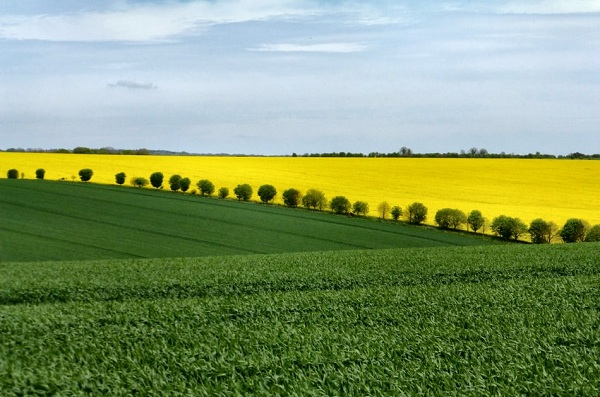
\includegraphics[width=\textwidth,height=\textheight,keepaspectratio]{img/in1.jpg}
            \caption{}
        \end{subfigure}
        \begin{subfigure}[b]{0.3\textwidth}
            \centering
            \includegraphics[width=\textwidth,height=\textheight,keepaspectratio]{img/out1_3.jpg}
            \caption{}
        \end{subfigure}
         \begin{subfigure}[b]{0.3\textwidth}
            \centering
            \includegraphics[width=\textwidth,height=\textheight,keepaspectratio]{img/out1_4.jpg}
            \caption{}
        \end{subfigure}
        \caption{(a) Ảnh gốc; (b) Ảnh sau khi phân vùng với $k=3$; (c) Ảnh sau khi phân vùng với $k=4$}
    \end{figure}

    \begin{figure}[H]
        \centering
        \begin{subfigure}[b]{0.3\textwidth}
            \centering
            
\includegraphics[width=\textwidth,height=\textheight,keepaspectratio]{img/in4.jpg}
            \caption{}
        \end{subfigure}
        \begin{subfigure}[b]{0.3\textwidth}
            \centering
            \includegraphics[width=\textwidth,height=\textheight,keepaspectratio]{img/out4_3.jpg}
            \caption{}
        \end{subfigure}
         \begin{subfigure}[b]{0.3\textwidth}
            \centering
            \includegraphics[width=\textwidth,height=\textheight,keepaspectratio]{img/out4_6.jpg}
            \caption{}
        \end{subfigure}
        \caption{(a) Ảnh gốc; (b) Ảnh sau khi phân vùng với $k=3$; (c) Ảnh sau khi phân vùng với $k=6$}
    \end{figure}

    \begin{figure}[H]
        \centering
        \begin{subfigure}[b]{0.3\textwidth}
            \centering
            \includegraphics[width=\textwidth,height=\textheight,keepaspectratio]{img/cat.jpg}
            \caption{}
        \end{subfigure}
        \begin{subfigure}[b]{0.3\textwidth}
            \centering
            \includegraphics[width=\textwidth,height=\textheight,keepaspectratio]{img/cat_5.jpg}
            \caption{}
        \end{subfigure}
         \begin{subfigure}[b]{0.3\textwidth}
            \centering
            \includegraphics[width=\textwidth,height=\textheight,keepaspectratio]{img/cat_10.jpg}
            \caption{}
        \end{subfigure}
        \caption{(a) Ảnh gốc; (b) Ảnh sau khi phân vùng với $k=5$; (c) Ảnh sau khi phân vùng với $k=10$}
    \end{figure}

    \subsection{Đánh giá chất lượng ảnh sau khi phân vùng}
    \subsubsection{Sai số toàn phương trung bình}
    Sai số toàn phương trung bình (Mean squared error) là trung bình của bình phương các sai số, tức là sự khác biệt giữa các ước lượng và những gì được đánh giá. MSE được sử dụng như một độ đo tiêu chuẩn trong xử lý hình ảnh cho biết hỉnh ảnh đầu ra bị lệch bao nhiêu so với ảnh gốc. MSE càng nhỏ thì chất lượng ảnh đầu ra càng tốt.

    Công thức của MSE với ảnh có kích cỡ $m \times n$, $I$ là ảnh gốc và $K$ là ảnh đầu ra:
    $$MSE = \frac{1}{mn} \sum\limits_{i=0}^{m-1} \sum\limits_{j=0}^{n-1} [I(i,j) - K(i,j)]^2$$

    \begin{table}[H]
        \centering
        \begin{tabular}{c|c|c}
            Ảnh & $k = 3$ & $k = 4$ \\
            \hline
            MSE & 78.24 & 74.88
        \end{tabular}
        \caption{Bảng giá trị MSE của Hình 8}
    \end{table}

    \begin{table}[H]
        \centering
            \begin{tabular}{c|c|c}
                Ảnh & $k = 3$ & $k = 6$ \\
                \hline
                MSE & 93.31 & 77.80
            \end{tabular}
        \caption{Bảng giá trị MSE của Hình 9}
    \end{table}

    \begin{table}[H]
        \centering
        \begin{tabular}{c|c|c}
            Ảnh & $k = 5$ & $k = 10$ \\
            \hline
            MSE & 67.26 & 35.04
        \end{tabular}
        \caption{Bảng giá trị MSE của Hình 10}
    \end{table}

    \subsubsection{Tỉ số tín hiệu cực đại trên nhiễu}
    Tỉ số tín hiệu cực đại trên nhiễu (Peak signal-to-noise ratio) là tỉ lệ giữa giá trị năng lượng tối đa của một tín hiệu và năng lượng nhiễu ảnh hướng đến độ chính xác của thông tin. PSNR được sử dụng để đo chất lượng tín hiệu khôi phục của các thuật toán nén có mất mát dữ liêu. PSNR càng lớn thì chất lượng ảnh đầu ra càng tốt.
    
    Công thức của PSNR được xác định thông qua MSE với ảnh có kích cỡ $m \times n$, $I$ là ảnh gốc và $K$ là ảnh đầu ra:
    $$PSNR = 20 \cdot log_{10}\left( \frac{255}{\sqrt{MSE}} \right)$$

    Giá trị thông thường của PSNR nằm từ 30 đến 50 dB, giá trị càng cao thì càng tốt.

    \begin{table}[H]
        \centering
        \begin{tabular}{l|l|l}
            Ảnh & $k = 3$ & $k = 4$ \\
            \hline
            PSNR & 29.20 dB & 29.39 dB
        \end{tabular}
        \caption{Bảng giá trị PSNR của Hình 8}
    \end{table}

    \begin{table}[H]
        \centering
        \begin{tabular}{c|c|c}
            Ảnh & $k = 3$ & $k = 6$ \\
            \hline
            PSNR & 28.43 dB & 29.22 dB
        \end{tabular}
        \caption{Bảng giá trị PSNR của Hình 9}
    \end{table}

    \begin{table}[H]
        \centering
        \begin{tabular}{c|c|c}
            Ảnh & $k = 5$ & $k = 10$ \\
            \hline
            PSNR & 29.85 dB & 32.68dB
        \end{tabular}
        \caption{Bảng giá trị PSNR của Hình 10}
    \end{table}

    Qua đây ta có thể thấy được rằng tăng số cụm có thể tăng chất lượng ảnh đầu ra.
    
    \section{Kết luận}
    \label{sec:summary}
    Qua đề tài này chúng tôi đã nghiên cứu và hiểu được về bài toán phân cụm, các độ đo, phương pháp cũng như ưu nhược điểm của từng phương pháp. Chúng tôi cũng đã đi sâu hơn một chút và nghiên cứu cụ thể về thuật toán K-Means và cách khởi tạo ta số cụm tối ưu bằng phương pháp Elbow. Cuối cùng, chúng tôi đã áp dụng vào bài toán phân vùng ảnh và đánh giá được chất lượng hình ảnh đầu ra qua 2 công thức MSE và PSNR.

    \section{Tài liệu tham khảo}
    \begin{enumerate}
        \item Jasmine Irani, Nitin Pise, Madhura Phatak(2016): Clustering Techniques and the Similarity Measures used in Clustering: A Survey.
        \item Nameirakpam Dhanachandra, Khumanthem Manglem and Yambem Jina Chanu(2015): Image Segmentation using K-means Clustering Algorithm and Subtractive Clustering Algorithm.
        \item Mahamed G.H. Omran, Andries P Engelbrecht and Ayed Salman(2007): An Overview of Clustering Methods
        \item Peak signal-to-noise ratio: \url{https://en.wikipedia.org/wiki/Peak\_signal-to-noise\_ratio}
        \item Mean squared error: \url{https://en.wikipedia.org/wiki/Mean\_squared\_error}
        \item Metric space: \url{https://en.wikipedia.org/wiki/Metric\_space}
        \item Phương pháp Elbow: \url{https://phamdinhkhanh.github.io/deepai-book/ch\_ml/KMeans.html#phuong-phap-elbow-trong-lua-chon-so-cum}
    \end{enumerate}
\end{document}

